\documentclass[11pt]{book} 

\usepackage[paperheight=9in,paperwidth=7in]{geometry}

\usepackage{amsmath, amsthm}
\usepackage{amssymb}
\usepackage{color}
\usepackage{tikz}
\usepackage{pgfplots}
\usetikzlibrary{arrows}
\usepackage{hyperref}

\usepackage{graphicx}


\hypersetup{
    colorlinks,
    citecolor=black,
    filecolor=black,
    linkcolor=black,
    urlcolor=black
}
\definecolor{dandelion}{RGB}{240,255,48}

\newcommand{\hilight}[1]{\colorbox{yellow}{#1}}
\usepackage[english]{babel}

\addto\captionsenglish{
  \renewcommand{\contentsname}%
    {Contents}%
}

\usepackage{xcolor}

\newcommand{\highlight}[1]{%
  \colorbox{yellow!50}{$\displaystyle#1$}}

\newtheorem{theorem}{Theorem}
\newtheorem{prop}{Proposition}


\newenvironment{definition}[1][Definition]{\begin{trivlist}
\item[\hskip \labelsep {\bfseries #1}]}{\end{trivlist}}
\newtheorem{example}{Example}
\numberwithin{example}{chapter} 



             % Book class in 11 points
\parindent0pt  \parskip10pt             % make block paragraphs
\raggedright                            % do not right justify

\title{\bf Open Calculus}    % Supply information
\author{Editor-In-Chief: Adam Cross}   
          %   for the title page.
\date{\today}                           %   Use current date. 

% Note that book class by default is formatted to be printed back-to-back.

\usepackage[dvipsnames,prologue,table]{pstricks}
\usepackage{pst-text}
\usepackage{pst-char}
\usepackage{pst-grad}



\begin{document}  
\frontmatter  

%\newgeometry{margin=0in}
%\thispagestyle{empty}
%\setlength\parindent{0pt}
%\restoregeometry


\clearpage
\pagenumbering{roman}
                          % only in book class (roman page #s)
\maketitle                              % Print title page.


\thispagestyle{empty}
%% copyrightpage
\begingroup
\footnotesize
\parindent 0pt
\parskip \baselineskip

This work is subject to the GNU Free Documentation License (version 1.3) with the following additional clause: none of the major publishing houses may distribute this work commercially.

Complete license information is available at smartifybooks.com.

In particular, you may freely copy this work and you may distribute it for free or commercially (except major publishers), and you may edit this work to create your own fork of the project, but any such fork is subject to the same license.  


\vfill

Smartify Books, \\
Baton Rouge, LA \\
\texttt{smartifybooks.com}

%%%%{\LARGE\plogo}
\vspace*{2\baselineskip}


\endgroup
\clearpage

\thispagestyle{empty}

\chapter*{Contributors}

\section*{Adam Cross: Editor-in-Chief}

\begin{tabular}{lp{7cm}}
\raisebox{-.6\height}{
\includegraphics[width=2in]{AdamCross_pic.jpg}} & PhD student at LSU.  Calculus teacher.  Author of \textit{A Quick Tour of Fourier Series and Lie Groups}.
\end{tabular}




\clearpage






\tableofcontents                        % Print table of contents








\mainmatter                             % only in book class (arabic page #s)

\pagenumbering{arabic}

\part{A Part Heading}                   % Print a "part" heading



\chapter{Limits}     

\section{Introduction to Limits}

Everything in calculus is a limit, and a thorough understanding of limits is possibly the most challenging aspect of a first course in calculus.  But it is well worth your trouble to learn it, because later when you want to understand derivatives and integrals, well, those things are limits too.  

The basic idea of limits is simple.  If you have some function $f$, you ask yourself what value $f(x)$ is approaching as $x$ gets closer and closer to some number $a$.  The notation we use for that is $$\lim_{x\to a} f(x)$$.  You should learn that notation and learn how to say it out loud.  It is read ``the limit of f of x as x approaches a''.  Or you could also say ``as x goes to a''.  

Spoiler alert: when $f$ is \emph{continuous}, then $$\lim_{x\to a} f(x)$$ is just $f(a)$.  Think about that for a moment and convince yourself that it's not at all surprising.  Imagine $f(x)=x^2$.  Ask yourself what value $f(x)$ is approaching as $x$ goes to $2$.  Obviously, $f(x)$ is going to 4.

Limits are tricky when the functions are not continuous.  And students, I promise you we don't just make up pointless difficult ideas for no reason.  Derivatives are limits, and when we start computing derivatives, you usually won't be able to just plug in $x=a$ and see what the number is because usually if you plug in $x=a$ you'll get $0/0$, which is nonsense.  So you have to understand limits when the function \hilight{is not continuous}.


\begin{example} Consider the function $f$ in the graph. What is $\lim_{x\to 2} f(x)$?

\begin{center}
\begin{tikzpicture}
  \draw[<->] (-3,0) -- (3,0) node[right] {$x$};
  \draw[<->] (0,-3) -- (0,3) node[above] {$y$};
\draw (-0.1,2) -- (.1,2);
\draw (-0.1,1) -- (.1,1);
\draw (-0.1,-2) -- (.1,-2);

\node at (2,3) {$f$};

\node at (2,-0.4) {$2$};



\draw (2,-.2) -- (2,0.2);

\node at (-0.4,2) {$4$};
\node at (-0.4,1) {$2$};


\draw[scale=1,domain=-3:2,smooth,variable=\x,blue] plot ({\x},{(2/3.33)*(-(\x^3/3-\x^2/2-2*\x+2)+2)});
\draw[xscale=1,domain=2:4,smooth,variable=\x,blue] plot ({\x},{4-\x});

\draw (2,2) circle[radius=3pt];
\fill[white] (2,2)  circle[radius=3pt];

\fill[black] (2,1)  circle[radius=3pt];


\end{tikzpicture}


\end{center}

\end{example}


 The empty dot at $(2,4)$ means there is a hole in the graph at that point.  The filled-in dot at $(2,2)$ means that $f(2)=2$.  But when we evaluate $\lim_{x\to 2} f(x)$ the actual value at $x=2$ doesn't matter.  All that matters is where $f(x)$ is going when $x$ goes to 2.
 
 We haven't defined limits yet, but we will.  In the meantime, we hope you can see that if $x$ is near 2 (but not equal to 2) then $f(x)$ is near 4.  Understanding the idea of that is very imporant to your success in calculus.    

\section{The Formal Definition of a Limit}

We will present the formal definition of a limit in a very traditional way.  It will probably seem very confusing at first, but we hope that in time you will see that it's just a mathematical way to say what we illustrated in the previous section. 

\begin{definition}
For any function $f$, we say the limit as $x$ approaches $a$ of $f(x)$ equals $L$, and we write 
$$\lim_{x\to a}f(x)=L,$$ 
if for any $\epsilon>0$ there exists $\delta>0$ so that for all $x$ where $0< |x-a|<\delta$ we have $|f(x)-L|<\epsilon$.  
\end{definition}

The use of $\epsilon$ and $\delta$ in this definition is very customary.  They are Greek letters, but you shouldn't be alarmed.  They are just used to mean small numbers.  In words, the definition means that $f(x)$ is close to $L$ when $x$ is close to $a$.  

But ``close to'' is vague, right?  What does ``close to'' mean?  Mathematicians don't like to be vague.  We like to be exactly precise so there is no room for misunderstanding.  

The way we specify that $x$ is close to $a$ is by saying that $|x-a|<\delta$.  You should understand that $|x-a|$ is a distance.  It's the distance between $x$ and $a$.  The expression $|x-a|<\delta$ means that the distance between $x$ and $a$ is not bigger than $\delta$.  

The same is true of $|f(x)-L|<\epsilon$.  The expression   $|f(x)-L|$ is a measure of distance, and saying $|f(x)-L|<\epsilon$ means that the distance between $f(x)$ and $L$ is less than $\epsilon$.  

Study those ideas. Understand them.  

Thus, the definition of the limit means that when $x$ is close enough to $a$, it follows that $f(x)$ is close enough to $L$.  And what does ``close enough'' mean?  It means you can make it as small as you want.  No matter how close you want it, you can make $f(x)$ that close to $L$ by making $x$ close enough to $a$.  

And we always assume $x\neq a$.  Note that condition in the definition of the limit: for all $x$ where $\highlight{0< |x-a|}<\delta$ we have $|f(x)-L|<\epsilon$.  We assume $0<|x-a|$ because we want to allow the possibility that $f(a)\neq \lim_{x\to a} f(x)$.  Of course, those two things are equal when $f$ is continuous, and that is the definition of continous, but we don't want to study just continuous function.  


\section{Topology for Calculus, Lesson 1}



An ``open interval'' is an elementary idea.  We say an interval $(a,b)$ is open when it does not include its endpoints.  Now we define a more general notion of ``open''.  




\begin{definition}
A set $U$ in the real numbers is \emph{open} if for any element $x$ in $U$ there is an $\epsilon$ small enough so that $(x-\epsilon , x+\epsilon)$ is contained in $U$.  


\end{definition}



This is best illustrated with examples.  

\begin{example}
Is an ``open interval'' \emph{ open} according to this definition?  (If not, that would be really confusing, but let's make sure.)
\end{example}

Refer to the picture.  For any $x$ in the interval, you can find a small $\epsilon$ so that the small open interval $(x-\epsilon , x+\epsilon)$ is contained inside $(a,b)$. 




\begin{center}
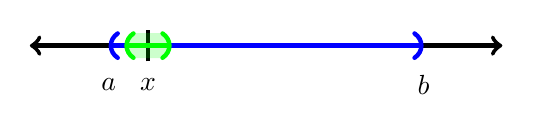
\begin{tikzpicture}
\draw[<->, ultra thick] (-3,0) -- (3,0) ;
\draw[(-), ultra thick, blue] (-2,0) -- (2,0);
\node[color=black] at (-2,-.5) {$a$};
\node[color=black] at (2,-.5) {$b$};

\draw[ultra thick] (-1.5,-.2) -- (-1.5,.2) ;
\node[color=black] at (-1.5,-.5) {$x$};

\draw[(-), green, ultra thick] (-1.8,0) -- (-1.2,0);
\fill[opacity = 0.2, green,rounded corners=1ex] (-1.8,.16) -- (-1.8, -.16) -- (-1.2, -.16) -- (-1.2,.16) -- cycle;

\end{tikzpicture}
\end{center}


So yes, intervals that are open in the ordinary sense are open in the sense we just defined.  


\begin{example}
Is a ``closed interval'' $[a,b]$ also \emph{open}?  Note that a closed interval includes its end points.

\end{example}

Here the answer is no because any open interval around $a$ no matter how small will contain values not in $[a,b]$.  It will contain some numbers less than $a$, and those are not in $[a,b]$.  There's a similar problem at $b$.  



\begin{center}
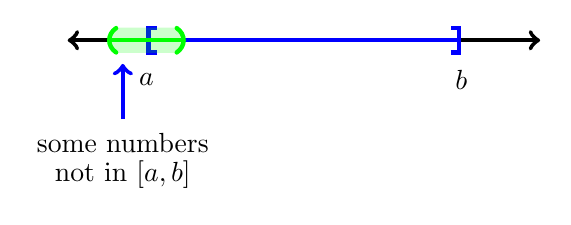
\begin{tikzpicture}
\draw[<->, ultra thick] (-3,0) -- (3,0) ;

\draw[[-, ultra thick, blue] (-2,0) -- (2,0);

\draw[[-, ultra thick, blue] (2,0) -- (-2,0);

\node[color=black] at (-2,-.5) {$a$};
\node[color=black] at (2,-.5) {$b$};


\draw[(-), green, ultra thick] (-2.5,0) -- (-1.5,0);

\fill[opacity = 0.2, green,rounded corners=1ex] (-2.5,.16) -- (-2.5, -.16) -- (-1.5, -.16) -- (-1.5,.16) -- cycle;


\draw[->, ultra thick, blue] (-2.3,-1) -- (-2.3,-.3);
\node at (-2.3,-1.3) {some numbers};
\node at (-2.3,-1.7) {not in $[a,b]$};

\end{tikzpicture}
\end{center}



\begin{example}
Is $(-1,1)\cup (3,4)$ open?  
\end{example}

Yes, a union of open intervals is open.

\begin{example}
Is the set $\mathbb{Z}$ of integers open?
\end{example}

No.  Any open interval around an integer contains numbers that are not integers.  Imagine a small interval around the number 1.  Students are sometimes tempted to say a set is ``closed'' when it is not open.  That's not correct.  We don't say a set is closed when it's not open.  In math, \emph{closed} has a different meaning.  


\begin{definition}
The \emph{preimage} $f^{-1}(U)$ is the set of all points $x$ where $f(x)$ is in $U$.
\end{definition}


Note that $f$ does not have to have an inverse, and here $f^{-1}$ does not mean the inverse in that sense, but they are related ideas.  When talking about preimages, we always put a \emph{set} inside $f^{-1}$, like $f^{-1}(U)$.

\begin{example}
Let $f(x)=\sin(x)$.  What is $f^{-1}(0,\infty)$?  Hint: This is exactly the same as asking to solve the inequality $f(x) >0$.
\end{example}


\begin{center}
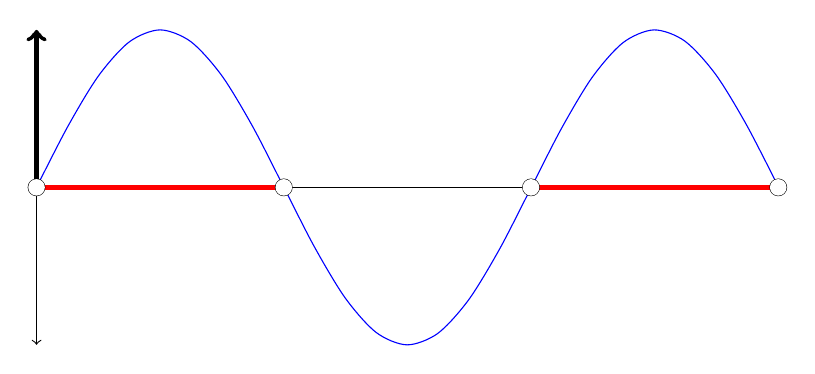
\begin{tikzpicture}
  \draw[<->] (-0.1,0) -- (9.41,0);
  \draw[<->] (0,-2) -- (0,2) ;

  \draw[->, ultra thick] (0,0) -- (0,2);

\draw[ultra thick, red] (0,0) -- (3.14,0);

\draw[ultra thick, red] (2* 3.14,0) -- (3*3.14,0);


\draw[yscale=2,domain=-0:9.41,smooth,variable=\x,blue] plot ({\x},{sin(\x r)});

\draw (0,0) circle[radius=3pt];
\fill[white] (0,0)  circle[radius=3pt];

\draw (3.14,0) circle[radius=3pt];
\fill[white] (3.14,0)  circle[radius=3pt];

\draw (3*3.14,0) circle[radius=3pt];
\fill[white] (3*3.14,0)  circle[radius=3pt];

\draw (2*3.14,0) circle[radius=3pt];
\fill[white] (2*3.14,0)  circle[radius=3pt];

\end{tikzpicture}
\end{center}






In the image we shaded $(0,\infty)$ along the y-axis.  We see $(0,\pi)$ and $(2\pi,3\pi)$ are both in $f^{-1}(0,\infty)$.  Those are both open intervals.  Since $\sin(x)$ just repeats the same wave over and over, 

$$f^{-1}(0,\infty) = \cdots (-4\pi,-3\pi)\cup (-2\pi,-\pi) \cup  (0,\pi) \cup  (2\pi,3\pi) \cup  (5\pi,6\pi) \cdots $$

This set $f^{-1}(0,\infty)$ is open.  It's an infinite union of open intervals.  


\begin{example}
Still considering $f(x)=\sin(x)$, what is $f^{-1}[0,1]$?  This is exactly the same as solving the inequality $0\leq f(x) \leq 1$.  
\end{example}

The only difference between this example and the last one is that now the preimage $f^{-1}[0,1]$ contains the end points.  

$$f^{-1}[0,1] = \cdots [-4\pi,-3\pi]\cup [-2\pi,-\pi] \cup  [0,\pi] \cup  [2\pi,3\pi] \cup  [5\pi,6\pi] \cdots $$

When we take an open set $U$, the preimage $f^{-1}(U)$ is also open.  This is true in general.

\begin{theorem}
If $f$ is continuous (everywhere) and $U$ is open, then $f^{-1}(U)$ is open.
\end{theorem}

This is an \textbf{equivalent} formulation of the idea of continuity.  It's a more mature way to understand continuity.  


Let's discuss the intuitive idea.  Below is a graph of a continuous function and an open set $U$.  By the picture, it certainly looks like $f^{-1}(U)$ is open, yes?  

\begin{center}
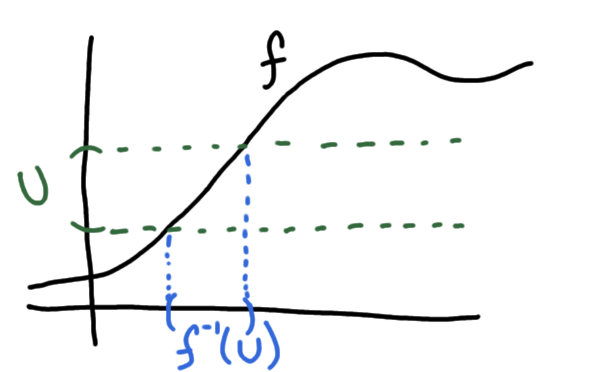
\includegraphics[width=4in]{toplec1_4.png}
\end{center}

Let's think a little about why it's open.  In the theorem, we do not assume that $U$ is an interval like in the picture.  To prove that $f^{-1}(U)$ is open, we need to show that for any $x$ in $f^{-1}(U)$ there is a little open interval around $x$ that is contained in $f^{-1}(U)$.

\begin{center}
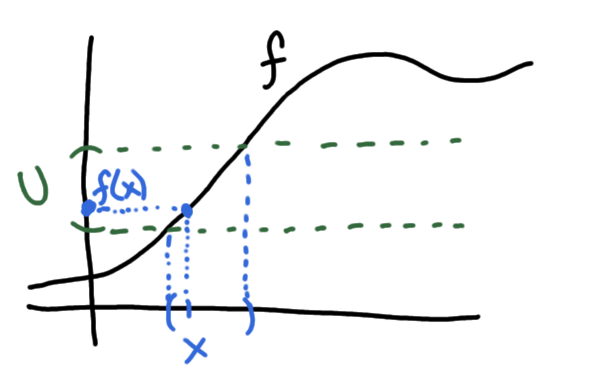
\includegraphics[width=4in]{toplec1_5.png}
\end{center}


An interval like that will look like this.  In the next image we see a little interval in red.  Any time a value $z$ is in that red interval, the function values $f(z)$ are inside $U$.  

\begin{center}
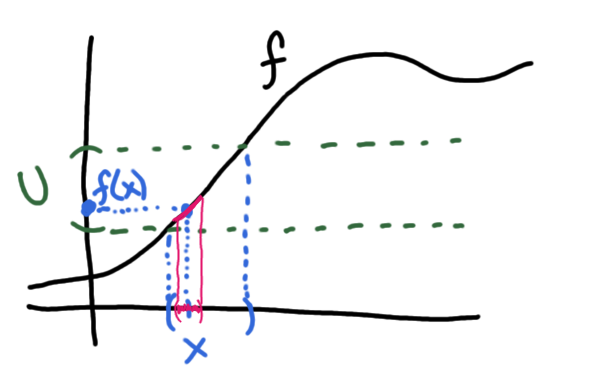
\includegraphics[width=4in]{toplec1_6.png}
\end{center}

Let's take one more step toward a formal proof.  Recall that $f(x)$ is in $U$ and $U$ is open.  That means we can produce a little open interval around $f(x)$ that is inside $U$.  In the next picture, we see a little $\epsilon$ interval $(f(x)-\epsilon, f(x)+\epsilon)$.  These are ``y''-values, so they are along the y axis.  

\begin{center}
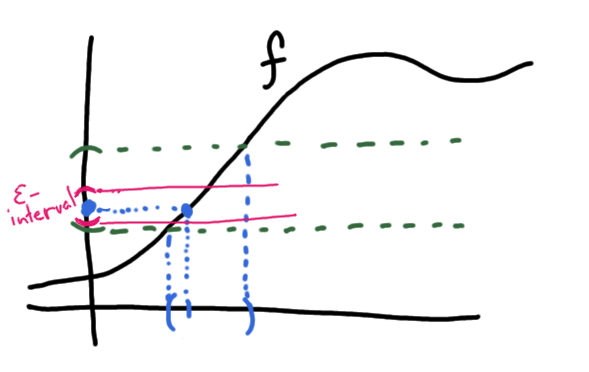
\includegraphics[width=4in]{toplec1_7.png}
\end{center}


Can we find a little $\delta$ interval around $x$ so that whenever $z$ is in  $(x-\delta,x+\delta)$ it follows that  $f(z)$ is in $(f(x)-\epsilon, f(x)+\epsilon)$?  If you are unsure, recall that this is exactly the definition of ``continuous at $x$''. 


\begin{center}
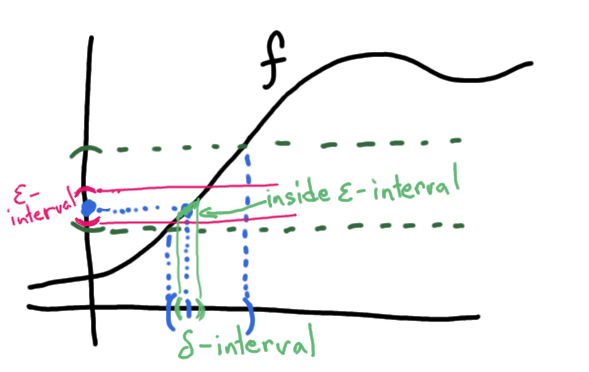
\includegraphics[width=4in]{toplec1_8.png}
\end{center}


If you understand this, then you will understand that the argument does not depend on our picture.  It works for any open set $U$.  


\subsection{The Role of Topology in Calculus}

Several of the most important ideas in calculus are basically topological---meaning to understand them the most natural thing is to use these ideas.  

Two of the most important examples: (1) the Intermediate Value Theorem, (2) the Extreme Value Theorem.


Here's why topology is useful in calculus.  So far we have defined everything \emph{pointwise}.  We defined continuity \emph{at x} and differentiability \emph{at x}, but some of the deeper theorems are about functions that are continuous \emph{everywhere}.  The Intermediate Value Theorem is not about any particular point, for example, and it's difficult to apply definitions of continuity that depend on some particular point $x$ when the theorem isn't about any particular point.  The alternative definition of continuous given in the theorem above allows us to take full advantage of functions that are continuous at every point in an interval.  

The ``topological'' method is an alternative point of view that will make the deeper theorems clearer if you can come to understand this point of view.  



\subsection{Exercises}

\begin{enumerate}
\item
Let $f(x)=\cos(x)$.  What is $f^{-1}(\{1\})$.  Here $\{1\}$ means the set containing just the number 1. Is $\{1\}$ open?  Is $f^{-1}(\{1\})$ open?




\item
Sketch an example of a function $f$ that is not continuous and some open set $U$ where $f^{-1}(U)$ is not open.  

\item
Refer to the theorem above about continuous functions.  If $U$ is not open, does that imply that $f^{-1}(U)$ is not open?

\item
Let $f(x)=x^2$.  Is $f$ continuous?  Let $U=(1,2)$. What is $f^{-1}(U)$?  Is $f^{-1}(U)$ open?  For this, don't just cite the theorem above, but convince yourself from the definition that it is open.



\end{enumerate}


\section{Extreme Value Theorem}


The Extreme Value Theorem is one of the foundational beams holding calculus up.  It's easy to state but very hard to prove (from the perspective of a calculus student).

\begin{theorem}
If $f$ is continuous on a closed interval $[a,b]$ then $f$ attains a global maximum and a global minimum.  
\end{theorem}

The word \emph{attains} in this theorem has a precise meaning.  We mean there is some $x$ in $[a,b]$ where $f(x)\leq f(a)$ for all $x\in [a,b]$.  We use \emph{attains} here to emphasize that $f$ actually equals its maximum at some point.  Contrast this with, for example, the function $arctan(x)$ which is bounded above by $\pi/2$ but never actually attains that value.  

In particular, this implies that $f$ is bounded.  

The Extreme Value Theorem is deep and topological in nature.  It's arguably the deepest theorem a calculus student would see, and therefore books tend to omit the proof.  

For the student who feels up to the challenge, we will try to push him in the right direction. 

The underlying idea behind the theorem is that a continuous function maps compact sets to compact sets, and in the real numbers, the compact sets are exactly the closed, bounded sets.  Thus, since $[a,b]$ is closed and bounded, $f([a,b])$ is also a closed, bounded set.

To prove the statement, however, we would make essential use of what \emph{compact} means.  We present the definition to give the reader an idea of the depth of the waters here.

\begin{definition}
A set $C$ is \emph{compact} if given any family $\{U_i\}$ of open sets that covers $C$, there is a finite subcollection $\{U_1, \ldots, U_p\}$ that covers $C$.  
\end{definition}

Here, ``cover'' means that $C$ is in the union.  


An alternative proof of the Extreme Value Theorem might rely on the statement that any sequence $\{x_i\}$ of points in $[a,b]$ has a convergent subsequence.  






\section{Exercises}

\begin{enumerate}

\item
Refer to the graphs.

\begin{center}
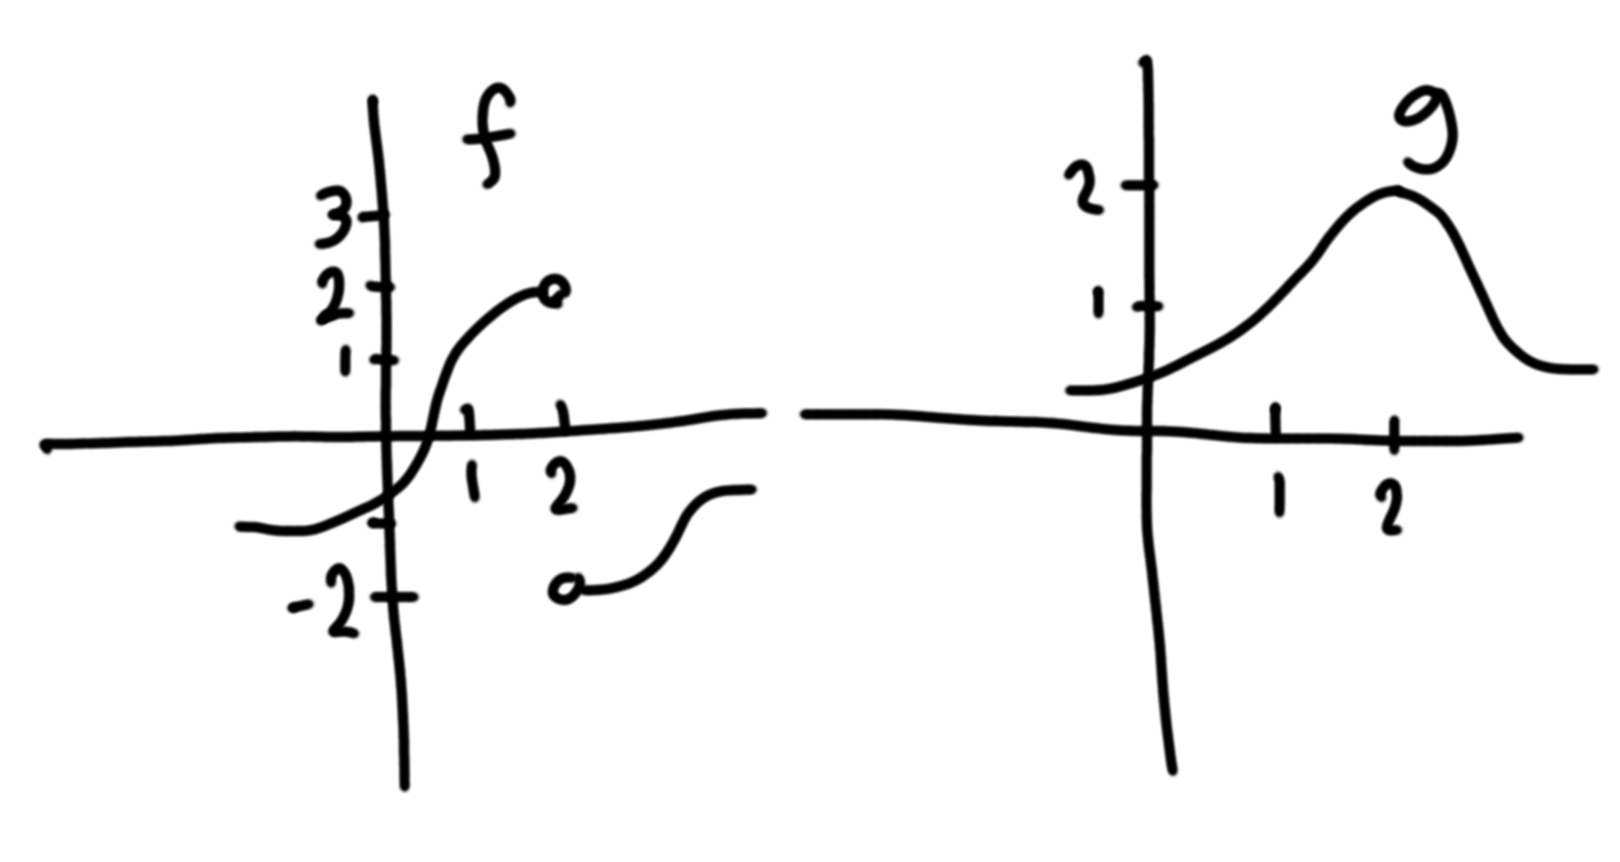
\includegraphics[width=4in]{limitExerciseImage1.png}
\end{center}

What is $\lim_{x\to 2} f(g(x))$?  What is $\lim_{x\to 2} g(f(x))$?




\item 

We will consider the limit $$\lim_{x\to 0} x^3.$$ 

\begin{enumerate}
\item 
Sketch a graph of $x^3$ around x=0 and draw two horizontal lines representing $\epsilon$ and $-\epsilon$. 



\item \label{b}
 What is the largest (most positive) value x can be so that   $x^3\leq \epsilon$?  
 

 
 \item \label{c}
  What is the most negative value x can be so that $x^3\geq -\epsilon$?



\item
What $\delta$ should we choose so that when $|x-0|<\delta$ we can be sure that $|x^3-0|<\epsilon$?  (Here we write the ``- 0'' part for emphasis so that it looks like the definition of a limit, but it can (and should) be omitted in most writing.  We want $\delta$ small so that $(x-\delta,x+\delta)$ is in the interval you identified in parts \ref{b} and \ref{c} above.



\item
If we require $|x^3-0|<1/1000$, how small does $|x|$ have to be?  



\end{enumerate}

\item

Explain in simple terms why $$\lim_{x\to 0} \frac{1}{x}$$ does not exist.  



\item
Explain in words why $$\lim_{x\to 0} x^2 \sin(2\pi/x)=0$$ (meaning the limit exists and is 0) but the limit $$\lim_{x\to 0} \sin(2\pi/x)$$ does not exist.  You are not required to write a proof, but explain what the essential difference is.









\end{enumerate}




\chapter{Derivatives}  

\section{Slope of the Tangent Line}

Given some function $f$, any two points on the curve determine a \emph{secant} line.  In the image below, $f(x)=\sin(x)$ and the two points pictured are $(\pi/2,1)$ and $(\pi/2+.5,\sin(\pi/2+.5))$.  


\begin{center}
\begin{tikzpicture}
  \draw[<->] (0,0) -- (6,0) node[right] {$x$};
  \draw[<->] (0,-1) -- (0,2) node[above] {$y$};

\draw (pi,-.2) -- (pi,.2); 
\node at (pi,-.5) {$\pi/2$};

%\draw (-1*2,1.629*2) -- (3*2,2*0.65);

\node[color=blue] at (2*pi/2,2*1) {\textbullet};
\node[color=red] at (2*2.07,2*.877) {\textbullet};
\draw[scale=2,domain=0:3,smooth,variable=\x,blue] plot ({\x},{sin(\x r)});

\draw[scale=2,domain=0:3,smooth,variable=\x,blue] plot ({\x},{1.38703-0.246392*\x});

\end{tikzpicture}
\end{center}

Recall how to conpute the slope of this line:

$$\frac{f(\pi/2+.5) - f(\pi/2)}{\pi/2+.5 - \pi/2}.$$
In this example, we think of $(\pi/2,1)$ as a fixed point we are interested in, and we pick another point close to it.  The $x$-coordinate differed by only a small number, 0.5.  It's traditional to use the letter $h$ to refer to that small number.  

If we choose an even smaller $h$, we get a different secant line.  Consider $h=0.3$.  In the next image, we have zoomed in close to $\pi/2$ and drawn the two secant lines given by $h=0.5$ and $h=0.3$.  


\begin{center}
\begin{tikzpicture}
\draw[<->] (-6,8) -- (6,8) node[right] {$x$};


%  \draw[<->] (0,-1) -- (0,2) node[above] {$y$};

%\draw (pi,-.2) -- (pi,.2); 
%\node at (pi,-.5) {$\pi/2$};

%\draw (-1*2,1.629*2) -- (3*2,2*0.65);

\node[color=blue] at (0,10) {\textbullet};


\node[color=red] at (10*.5,10*.877) {\textbullet};

\node[color=red] at (10*.3,10*.9553) {\textbullet};

\draw[scale=10,domain=-.5:.5,smooth,variable=\x,blue] plot ({\x},{sin((\x+pi/2) r)});

\draw[scale=10,domain=-.5:.5,smooth,variable=\x,blue] plot ({\x},{1.38703-0.246392*(\x+pi/2)});

\draw[scale=10,domain=-.5:.5,smooth,variable=\x,blue] plot ({\x},{1.23386-0.148878*(\x+pi/2)});


\end{tikzpicture}
\end{center}

Naturally, one might ask what happens as $h$ gets smaller and smaller.  Imagine the point at $(x+h,f(x+h))$ getting closer and closer to $(x,f(x)$.  What happens to the secant lines in the limit?  And what happens to the slope?  

In the example pictured, in the limit the secant lines go to a horizontal line.  We call this the tangent line.
\begin{center}
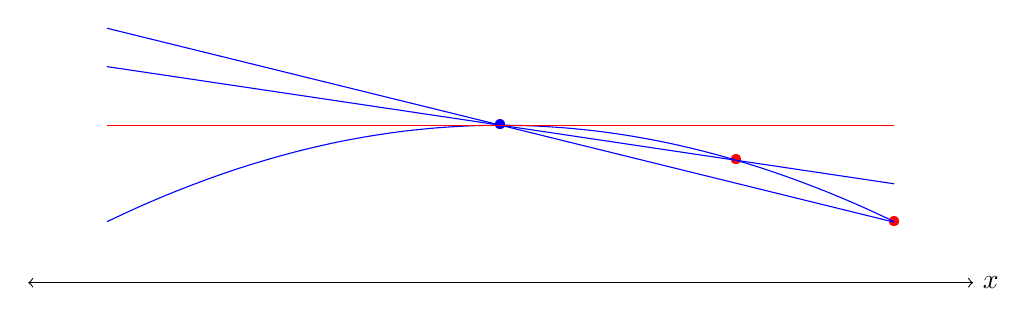
\begin{tikzpicture}
\draw[<->] (-6,8) -- (6,8) node[right] {$x$};


%  \draw[<->] (0,-1) -- (0,2) node[above] {$y$};

%\draw (pi,-.2) -- (pi,.2); 
%\node at (pi,-.5) {$\pi/2$};

%\draw (-1*2,1.629*2) -- (3*2,2*0.65);

\node[color=blue] at (0,10) {\textbullet};


\node[color=red] at (10*.5,10*.877) {\textbullet};

\node[color=red] at (10*.3,10*.9553) {\textbullet};

\draw[scale=10,domain=-.5:.5,smooth,variable=\x,blue] plot ({\x},{sin((\x+pi/2) r)});

\draw[scale=10,domain=-.5:.5,smooth,variable=\x,blue] plot ({\x},{1.38703-0.246392*(\x+pi/2)});

\draw[scale=10,domain=-.5:.5,smooth,variable=\x,blue] plot ({\x},{1.23386-0.148878*(\x+pi/2)});

\draw[scale=10,domain=-.5:.5,smooth,variable=\x,red] plot ({\x},{1});
\end{tikzpicture}
\end{center}


\begin{definition}
The \emph{tangent line of $f$ at $x$} is the limit of the secant line through $(x,f(x))$ and $(x+h,f(x+h))$ as $h$ goes to 0.  
\end{definition}

If the limit does not exist, then the tangent line is undefined.

In general the slope of the tangent line is the limit of the slope of the secant line:
$$\lim_{h\to 0} \frac{f(x+h)-f(x)}{h}$$




\begin{definition}
The \highlight{\emph{derivative of $f$ at $a$}} is 
$$f'(a)=\lim_{h\to 0} \frac{f(a+h)-f(a)}{h}$$
if the limit exists and is finite.
\end{definition}

If the limit doesn't exist or if it is infinite, we say the function is not \emph{differentiable} at $a$.

Students should memorize this definition.  It's very basic to an understanding of calculus.

We often use the notation $f'(x)$ for the derivative of $f$ at x.  We also use the notation $\frac{d}{dx}f(x)$ for the derivative of $f$ at $x$.  The two notations are used interchangeably.  Usually, when we use the $\frac{d}{dx}$ it's because we want to be explicit that we are taking the derivative \emph{with respect to $x$}.  We will talk about that more later.

In this section, we have learned one interpretation of the derivative of $f$ at $a$.  It is the slope of the tangent line at $a$.  We will learn some other interpretations in later sections.   

This expression 
$$\frac{f(x+h)-f(x)}{h}$$
is often called a \emph{difference quotient}.  As we have seen here, it's nothing but the familiar slope formula.  


\begin{example}
What is the derivative of $f(x)=x^{1/3}$ at 0?
\end{example}

\begin{center}
\begin{tikzpicture}
  \draw[<->] (-3,0) -- (3,0);
  \draw[<->] (0,-2) -- (0,2);
  
  \draw[<->,ultra thick, red] (0,-1) -- (0,1);

\node[color=blue] at (0,0) {\textbullet};

\draw[scale=2,domain=-1:1,samples=100,smooth,variable=\x,blue] plot ({\x},{\x^(1/3)});



\end{tikzpicture}
\end{center}


\begin{align*}
&\lim_{h\to 0}\frac{f(a+h)-f(a)}{h}\\
=&\lim_{h\to 0}\frac{h^{1/3}}{h}\\
=& \lim_{h\to 0} h^{-2/3}=\infty
\end{align*}

Since the limit is infinite, the derivative does not exist.  This corresponds to the vertical tangent line at 0.

\begin{example}
Let $f(x)=x^2$ with the domain $[-1,1]$.  What is $f'(1)$?

\end{example}



\section{Ways a Function Might Not be Differentiable}


In the previous section, we saw the function $f(x)=x^{1/3}$, which is not differentiable at 0 because the tangent line has infinite slope at that point.  

In this section, we will consder other ways a function may fail to be differentiable.  In all cases, however, this reduces to showing that
$$\lim_{h\to 0}\frac{f(a+h)-f(a)}{h}$$
is infinite or does not exist.

\subsection{A Sharp Point}

The function $f(x)=|x|$ is not differentiable at 0.  The intuitive reason is that $f$ has a point there.  You might say there is no way to define a tangent line at 0.  

That kind of reasoning may be acceptable in a high school calculus class, but at the college level, you should be able to show from the definition that the derivative does not exist.

\begin{example}
Show that function $f(x)=|x|$ is not differentiable at 0.
\end{example}

How do we start?  (Try to answer before you continue reading.)

We write down the definition of the derivative at 0:
$$f'(0) = \lim_{h\to 0}\frac{|0+h|-|0|}{h}= \lim_{h\to 0}\frac{|h|}{h}$$

One way a limit may fail to exist is if the left hand limit and the right hand limit are not the same.  Recall that when $h>0$ we can write $|h|=h$ and when $h<0$ we can write $|h|=-h$.  Thus
$$\lim_{h\to 0^+}\frac{|h|}{h}=\lim_{h\to 0+}\frac{h}{h}=1$$ 
and 
$$\lim_{h\to 0^-}\frac{|h|}{h}=\lim_{h\to 0+}\frac{-h}{h}=-1.$$ 



Since the left and right limits are not equal, the limit does not exist, so the derivative does not exist at 0.  

This argument is completely sufficient, but let's also think about secant lines.  If $h$ is any positive number, then the secant line through the points $(0,0)$ and $(h,|h|)$ is always $y=x$.  That's true no matter how small $h$ is, so long as it is positive. 


\begin{center}
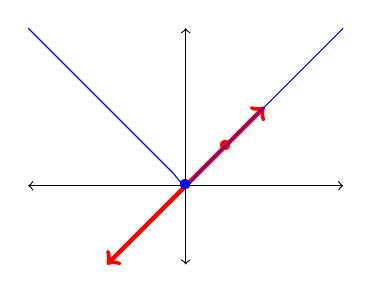
\begin{tikzpicture}
  \draw[<->] (-2,0) -- (2,0);
  \draw[<->] (0,-1) -- (0,2) ;


\draw[<->, ultra thick, red] (-1,-1) -- (1,1) ;

\node[color=blue] at (0,0) {\textbullet};

\node[color=red] at (.5,.5) {\textbullet};

\draw[scale=1,domain=-2:2,smooth,variable=\x,blue] plot ({\x},{abs(\x)});




\end{tikzpicture}
\end{center}


Now think about a negative $h$.  In this case, the secant line has slope -1 no matter how small $h$ is.



\begin{center}
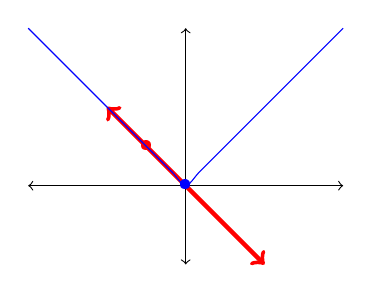
\begin{tikzpicture}
  \draw[<->] (-2,0) -- (2,0);
  \draw[<->] (0,-1) -- (0,2) ;


\draw[<->, ultra thick, red] (-1,1) -- (1,-1) ;

\node[color=blue] at (0,0) {\textbullet};

\node[color=red] at (-.5,.5) {\textbullet};

\draw[scale=1,domain=-2:2,smooth,variable=\x,blue] plot ({\x},{abs(\x)});
\end{tikzpicture}
\end{center}
So the secant lines don't approach any single tangent line.  

\subsection{Oscillating Secant}


Consider $f(x)=x\sin(1/x)$.  This function oscillates infinitely many times between the two lines $y=x$ and $y=-x$ so that around $x=0$ you can't even really graph it, but we can give the idea of it in the following image.



\begin{center}
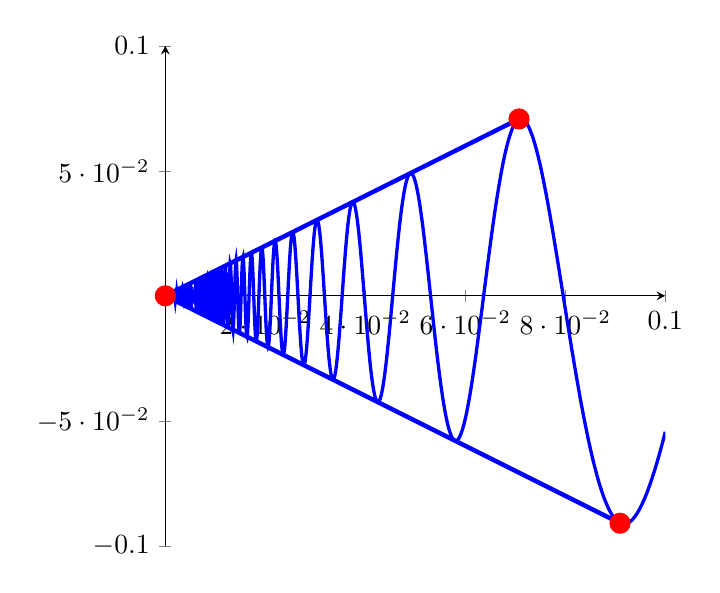
\begin{tikzpicture}


%\draw[scale=100,domain=0.001:0.1,smooth,samples=50,variable=\x,blue] plot ({\x},{1/100*sin((1/\x) r)});

\begin{axis}[samples=1000,
axis x line=center,
y=12.5in,
x=25in,
axis y line=center,
xmin=0,
xmax=0.1,
ymin=-.1,
ymax=.1,restrict y to domain =-2:2]
\addplot[very thick,blue,domain=0.0004:.1]plot (\x, {\x*sin((1/\x r))});

\addplot[ultra thick,blue,domain=0:0.070735]plot (\x, {\x});

\addplot[ultra thick,blue,domain=0:0.090945681766]plot (\x, {-\x});


\end{axis}
\draw[red,fill=red] (0.070735*25in,1.25in +12.5*0.070735 in) circle (.05in);

\draw[red,fill=red] (0,1.25in) circle (.05in);

\draw[red,fill=red] (0.090945681766*25in,.113 in) circle (.05in);



\end{tikzpicture}
\end{center}

No matter how much you zoom it, it still looks basically the same: the oscillations bunch up tighter and tighter at 0.  Also, no matter how close we zoom in, there are some values of $x$ where $\sin(1/x)=1$ and others where $\sin(1/x)=-1$.  Those are places where $x\sin(1/x)$ touches the bounding lines $y=x$ and $y=-x$.

In the figure, we illustrated two secant lines.  At $x_n=\frac{1}{\pi(4n+1)}$ we have $f(x_n)=x_n$.  In the figure, we have drawn $(x_2,f(x_2)$ and you can see that the secant line between $(0,0)$ and $(x_2,f(x_2)$ has slope 1.  

However, at $z_n=\frac{2}{\pi(4n-1)}$ we have $f(z_n)=-z_n$.  We have drawn the point $(z_2,f(z_2)$  The secant line between $(0,0)$ and $(z_2,f(z_2)$ has slope -1.  

The derivative of $f$ at 0 does not exist in this example because no matter how close $h$ is to 0, there are always some values of $h$ where 
$$\frac{f(h)-f(0)}{h}=1$$
and some values of $h$ where 
$$\frac{f(h)-f(0)}{h}=-1.$$
Since they are not zeroing in toward a single number, the limit does not exist.  

Contrast with the function $f(x)=x^2\sin(1/x)$ which \emph{is} differentiable at 0.  

\section{The Product Rule}

\begin{prop}
If $f$ and $g$ are differentiable at $a$ then 
$$\frac{d}{dx}[f(x)g(x)]=f'(a)g(a)+f(a)g'(a)$$

\end{prop}



\begin{center}
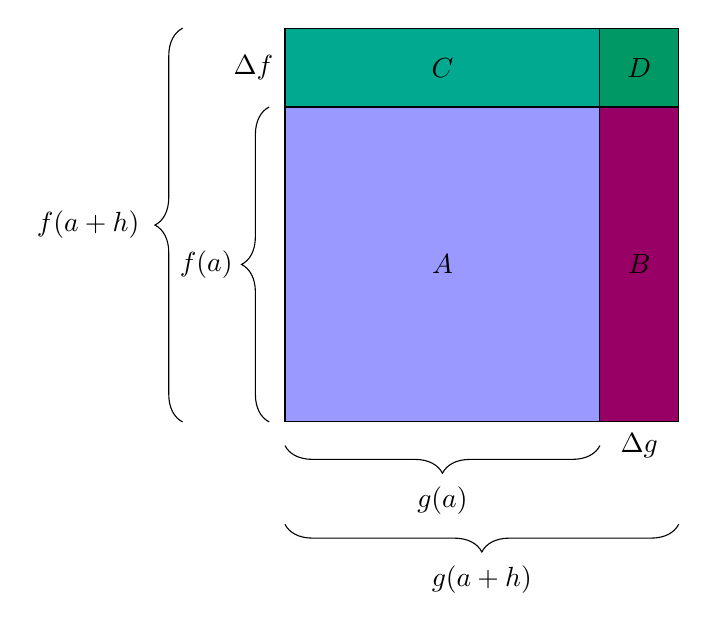
\begin{tikzpicture}
\filldraw[blue!40!white, draw=black] (0,0) rectangle (4,4);
\filldraw[blue!40!red, draw=black] (4,0) rectangle (5,4);

\filldraw[blue!40!green, draw=black] (0,4) rectangle (4,5);

\filldraw[cyan!40!green, draw=black] (0,4) rectangle (4,5);

\filldraw[blue!40!green, draw=black] (4,4) rectangle (5,5);

\draw [decorate,decoration={brace,amplitude=10pt}] (-.2,0) -- (-.2,4);

\draw [decorate,decoration={brace,amplitude=10pt}] (-1.3,0) -- (-1.3,5);

\draw [decorate,decoration={brace,amplitude=10pt,mirror}] (0,-.3) -- (4,-.3);

\draw [decorate,decoration={brace,amplitude=10pt,mirror}] (0,-1.3) -- (5,-1.3);


\node at (-2.5,2.5) {$f(a+h)$};

\node at (-1,2) {$f(a)$};
\node at (2,-1) {$g(a)$};
\node at (2,2) {$A$};
\node at (-.4,4.5) {$\Delta f$};
\node at (4.5,2) {$B$};

\node at (2.5,-2) {$g(a+h)$};
\node at (2,4.5) {$C$};
\node at (4.5,4.5) {$D$};
\node at (4.5,-.3) {$\Delta g$};
\end{tikzpicture}
\end{center}


We present a visual argument that isn't completely general.  My students have found it illuminating. 

By definition, the derivative of $f(x)g(x)$ at $a$ is
$$\lim_{h\to 0}\frac{f(a+h)g(a+h)-f(a)g(a)}{h}$$
Let's assume for the moment that the numbers are all positive so we can illustrate them with rectangles as in the figure.

Observe that $f(a+h)g(a+h)$ is the combined area of the four rectangles A, B, C and D while $f(a)g(a)$ is the area of just rectangle A.  Therefore, $f(a+h)g(a+h)-f(a)g(a)$ is the area of B + C + D.  

Now, it's easy to see that $C=g(a)(f(a+h)-f(a))$ and $B=f(a)(g(a+h)-g(a))$ and $D=(f(a+h)-f(a))(g(a+h)-g(a))$.  To compute the limit above, we take 
$$\lim_{h\to 0} \frac{B+C+D}{h}.$$

Now, we see that 
$$\lim_{h\to 0} \frac{B}{h}=\lim_{h\to 0} \frac{f(a)(g(a+h)-g(a))}{h}=f(a)g'(a).$$
Similarly
$$\lim_{h\to 0} \frac{C}{h}=\lim_{h\to 0} \frac{g(a)(g(a+h)-g(a))}{h}=g(a)f'(a).$$
Finally
$$\lim_{h\to 0} \frac{D}{h}=\lim_{h\to 0} \frac{g(a+h)-g(a)}{h}(f(a+h)-f(a))=0.$$

Therefore the derivative at $a$ is $f(a)g'(a)+g(a)f'(a)$.

Note that to draw the visual in terms of areas of rectangles, we made assumptions about things being positive, but that really played no role in the argument.  $f(a+h)g(a+h)-f(a)g(a) = $

\section{The Chain Rule}


\begin{prop}
If $f$ and $g$ are differentiable then $\frac{d}{dx}f(g(x)) = f'(g(x))g'(x)$.
\end{prop}

\begin{example}

Compute the derivative $\frac{d}{dx}\sin(x^2)$.

The outside function in this composition is $f(x)=\sin(x)$.  The inside function is $g(x)=x^2$.  Thus $\frac{d}{dx}\sin(x^2) = f'(g(x))g'(x)= \cos(x^2)(2x)$.

\end{example}

The following proof sketch is intended to be illuminating rather than exactly precise.  An exactly precise proof would be written with $\epsilon$s and $\delta$s, but we think the student is more likely to undestand the idea presented this way.

\begin{proof}[Proof Sketch]

Since $g'(x)$ exists, for $h$ small, 
$$\frac{g(x+h)-g(x)}{h}\approx g'(x).$$

Here the $\approx$ symbol means ``is approximately''.  Therefore, 
$$g(x+h)-g(x)\approx hg'(x)$$
and 
$$g(x+h)\approx hg'(x)+g(x).$$

To compute the derivative of $f(g(x))$ at $x$, the difference quotient is $$\frac{f(g(x+h))-f(g(x))}{h}.$$
For $h$ small, 
$$ 
\frac{f(\highlight{g(x+h)})-f(g(x))}{h} \approx \frac{f(\highlight{g(x) + hg'(x)})-f(g(x))}{h}.$$
Observe we have just replaced $g(x+h)$ with $g(x) + hg'(x)$.  Next we multiply top and bottom by $g'(x)$ and we have 
\begin{equation} \label{3240972392408}
\frac{f(g(x) + hg'(x))-f(g(x))}{hg'(x)} g'(x).
\end{equation}

The quotient on the left in  (\ref{3240972392408}) almost has the form of a difference quotient.  As $h\to 0$, we also see that $hg'(x)\to 0$ so 
$$\lim_{h\to 0} \frac{f(g(x) + hg'(x))-f(g(x))}{hg'(x)}  = \lim_{h\to 0} \frac{f(g(x) + h)-f(g(x))}{h} = f'(g(x)).$$
Those limits are the same because it doesn't really matter what symbol appears in the highlighted portion of the difference quotient: 
$$\frac{f(g(x) + \highlight{hg\prime(x)})-f(g(x))}{\highlight{hg'(x)}}.$$
It only matters that those two numbers are the \emph{same} and that they are going to zero in the limit.  That's why we had to multiply and divide by $g'(x)$.  We needed to have the same number in those two highlighted positions.  

Thus $\frac{d}{dx}f(g(x)) = f'(g(x))g'(x)$.
\end{proof}

\section{Practice Quiz}

For the best learning experience, treat a practice quiz like an in-class quiz. Don't refer to other parts of the textbook.

\begin{enumerate}


\item Circle T for true or F for false:
\begin{enumerate}
\item T/F For any numbers $a$ and $b$, where $a<b$, there is a rational number $p/q$ so that $a<p/q<b$.

\item T/F The number $\sqrt{2}$ can be written as $p/q$ where $p$ and $q$ are both integers.

\item T/F The limit $\lim_{n\to \infty} (1+1/n)^{n}$ does not exist.

\item T/F It's possible to find a rational number as close to $\pi$ as you want.

\end{enumerate}


\item Compute the derivative.  

\begin{enumerate}
\item
$\frac{d}{dx} e^{\sin(x)}$
\item
$\frac{d}{dx} \ln(\cos(x))$
\item
$\frac{d}{dx} x^3\tan(x)$
\item
$\frac{d}{dx} \sin(x)^x$
\end{enumerate}




\item
Compute the derivative $\frac{d}{dx} \sin^{-1}(x)$ using the chain rule/implicit differentiation technique.  



\item Let's think about how to approximate $\sin(1^\circ)$.

\begin{enumerate}


\item  Since $1^\circ$ is close to $0^\circ$, we will find a tangent line at 0.  But why is $0^\circ$ any easier than $1^\circ$?



\item What is the slope of the tangent line at $0$?



\item What is the equation of the tangent line at $0$?



\item What is the value of the tangent line at $1^\circ$?  (Be sure to convert into radians.)



\item Why is your answer in the previous part a reasonable approximation to $\sin(1^\circ)$?

\end{enumerate}


\end{enumerate}



\section{Extreme Values}


We say a function $f$ has a \emph{local maximum} at a point $a$ if there is an interval $(a-\epsilon,a+\epsilon)$ around $a$ where $f(x)\leq f(a)$ for all $x$ in $(a-\epsilon,a+\epsilon)$ and in the domain of $f$. 

Another way to say this is $f(x)\leq f(a)$ in a neighborhood of $a$.  

A \emph{local maximum} is defined similarly.  


We say $f$ has a \emph{global maximum} at $a$ if $f(x)\leq f(x)$ for all $x$ in the domain of $f$.  

A \emph{global maximum} is defined similarly.  

\begin{example}

In the following example, $f$ is defined on $[-2.5,2]$.  There are local maxima at $a$ and $2$.  There are local minima at $b$ and $-2.5$.  The global max is at $a$.  The global min is at $-2.5$.  




\begin{center}
\begin{tikzpicture}
  \draw[<->] (-4,0) -- (3,0) node[right] {$x$};
  \draw[<->] (0,-1) -- (0,2) node[above] {$y$};

\draw (-.8685,-0.1) -- (-.8685,0.1)
node[below=0.1in] {$a$};

\draw (1.54,-0.1) -- (1.54,0.1)
node[below=0.1in] {$b$};

\draw (-2.5,-0.1) -- (-2.5,0.1)
node[below=0.1in] {$-2.5$};

\draw (2,-0.1) -- (2,0.1)
node[below=0.1in] {$2$};

\draw[scale=1,domain=-2.5:2,smooth,variable=\x,blue] plot ({\x},{1/5*(\x+2)*(\x-1)*(\x-2)});

\node[color=black] at (-2.5,2) {$f$};

\node[color=blue] at (-2.5,-1.57) {\textbullet};

\node[color=blue] at (2,0) {\textbullet};

\end{tikzpicture}
\end{center}

\end{example}


\begin{prop}
If $f$ is defined on an interval $[a,b]$ and $f$ has a local minimum or a local maximum at $c \in [a,b]$, where $c$ is not one of the endpoints, and if $f$ is differentiable at $c$ then $f'(c)=0$.   
\end{prop}

Why did we assume $c$ isn't an endpoint?  Consider $f(x)=x^2$ restricted to the domain $[-2,2]$.  Then $f$ has a local (and global) max at $x=2$, but the derivative at $2$ is $f'(2)=4$.  

\begin{center}
\begin{tikzpicture}
  \draw[<->] (-3,0) -- (3,0) node[right] {$x$};
  \draw[<->] (0,-1) -- (0,4.2) node[above] {$y$};
\draw (-2,-0.1) -- (-2,0.1)
node[below=0.1in] {-2};
\draw (2,-0.1) -- (2,0.1)
node[below=0.1in] {2};
\node[color=blue] at (-2,4) {\textbullet};
\node[color=blue] at (2,4) {\textbullet};
\draw[scale=1,domain=-2:2,smooth,variable=\x,blue] plot ({\x},{\x*\x});
\end{tikzpicture}
\end{center}

Is it possible that $f$ has a local maximum at $a$ but $f'(a)$ doesn't exist?  Consider $f(x)=|x|$, which has a local minimum at 0, but $f'(0)$ does not exist.  So we have to assume $f'(a)$ exists.  

\begin{center}
\begin{tikzpicture}
  \draw[<->] (-3,0) -- (3,0) node[right] {$x$};
  \draw[<->] (0,-1) -- (0,3) node[above] {$y$};
\draw (-2,-0.1) -- (-2,0.1)
node[below=0.1in] {-2};
\draw (2,-0.1) -- (2,0.1)
node[below=0.1in] {2};
\node[color=blue] at (-2,2) {\textbullet};
\node[color=blue] at (2,2) {\textbullet};
\draw[scale=1,domain=-2:2,smooth,variable=\x,blue] plot ({\x},{abs(\x)});
\end{tikzpicture}
\end{center}

\begin{proof}
Assume $f$ has a local maximum at $c$.  We consider the limit of $\frac{f(c+h)-f(c)}{h}$ as $h\to 0$ from the right and from the left.  

If $h>0$ and $h$ is small enough, then 
$$\frac{f(c+h)-f(c)}{h}\leq 0.$$
Consider the slope of the secant line in the following illustration.

\begin{center}
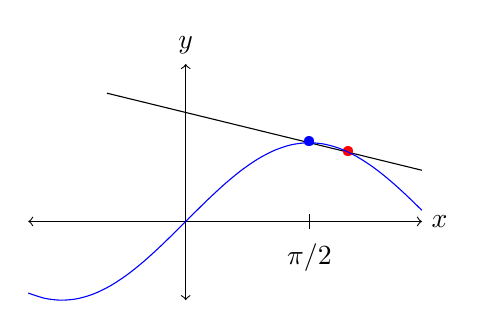
\begin{tikzpicture}
  \draw[<->] (-2,0) -- (3,0) node[right] {$x$};
  \draw[<->] (0,-1) -- (0,2) node[above] {$y$};

\draw (pi/2,-0.1) -- (pi/2,0.1)
node[below=0.1in] {$\pi/2$};

\draw (-1,1.629) -- (3,0.65);
\node[color=blue] at (pi/2,1) {\textbullet};
\node[color=red] at (2.07,.877) {\textbullet};
\draw[scale=1,domain=-2:3,smooth,variable=\x,blue] plot ({\x},{sin(\x r)});
\end{tikzpicture}
\end{center}

Thus $$\lim_{h\to 0^+}\frac{f(c+h)-f(c)}{h}\leq 0.$$

On the other hand, if $h<0$ then 
$$0\leq \frac{f(c+h)-f(c)}{h}.$$


\begin{center}
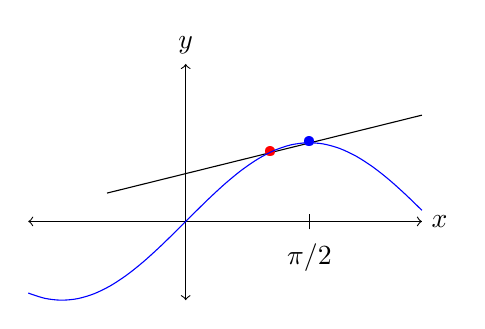
\begin{tikzpicture}
  \draw[<->] (-2,0) -- (3,0) node[right] {$x$};
  \draw[<->] (0,-1) -- (0,2) node[above] {$y$};

\draw (pi/2,-0.1) -- (pi/2,0.1)
node[below=0.1in] {$\pi/2$};

\draw (-1,.36) -- (3,1.35);
\node[color=blue] at (pi/2,1) {\textbullet};
\node[color=red] at (1.07,.877) {\textbullet};

\draw[scale=1,domain=-2:3,smooth,variable=\x,blue] plot ({\x},{sin(\x r)});
\end{tikzpicture}
\end{center}


Thus $$0\geq \lim_{h\to 0^-}\frac{f(c+h)-f(c)}{h}.$$
Since the limit exists, the right hand limit and the left hand limit are the same, so 
$$0\leq \lim_{h\to 0}\frac{f(c+h)-f(c)}{h} \leq 0$$
so $f'(c)=0$.

The argument is the same when $f$ has a local minimum at $c$.  The only difference is that the inequalities are flipped.  

\end{proof}








\chapter{Integrals}  



\end{document}                         